\documentclass[tikz,border=0pt]{standalone}
% Deterministic vector typography; formulas are compiled by XeLaTeX.
\usepackage{fontspec}
\IfFontExistsTF{Comic Sans MS}{\setmainfont{Comic Sans MS}}{\setmainfont{texgyreheros}[Extension=.otf,UprightFont=*-regular,BoldFont=*-bold,ItalicFont=*-italic,BoldItalicFont=*-bolditalic]}
\usepackage{amsmath}
\usepackage{fix-cm}
\usepackage{tikz}
\usetikzlibrary{arrows.meta,calc,positioning,shapes.geometric,backgrounds}
\definecolor{ink}{HTML}{2D2730}
\definecolor{muted}{HTML}{716771}
\definecolor{aubergine}{HTML}{563D5D}
\definecolor{coral}{HTML}{D66D75}
\definecolor{sage}{HTML}{7A9E7E}
\definecolor{ochre}{HTML}{C99331}
\definecolor{cream}{HTML}{FFF9F0}
\definecolor{lavender}{HTML}{F1EAF2}
\definecolor{mint}{HTML}{EDF4ED}
\definecolor{blush}{HTML}{FBECEE}
\definecolor{line}{HTML}{DED5DB}
\definecolor{green}{HTML}{4C7B00}
\definecolor{nvidiagreen}{HTML}{76B900}
\definecolor{graphite}{HTML}{242829}
\tikzset{
  every node/.style={font=\fontsize{8}{10.2}\selectfont,text=ink,inner sep=0pt},
  title/.style={font=\bfseries\fontsize{12}{14}\selectfont,anchor=west},
  sub/.style={font=\fontsize{7.5}{9.5}\selectfont,text=muted},
  label/.style={font=\bfseries\fontsize{8.6}{11}\selectfont},
  flow/.style={-{Latex[length=2.1mm,width=1.5mm]},line width=.9pt,draw=aubergine},
  control/.style={-{Latex[length=1.8mm,width=1.3mm]},line width=.8pt,dashed,draw=muted},
  card/.style={rounded corners=2.5mm,draw=line,line width=.65pt,fill=white},
  icon/.style={draw=aubergine,line width=.8pt},
}
\newcommand{\status}[2]{\node[sub,anchor=east,text=#2] at (16.83,#1) {ILLUSTRATIVE $\cdot$ NOT MEASURED};}
\newcommand{\step}[3]{\node[circle,fill=#3,text=white,font=\bfseries\fontsize{8}{8}\selectfont,minimum size=5mm] at (#1,#2) {};}
\newcommand{\thumbnail}[3]{%
  \begin{scope}[shift={(#1,#2)}]
    \fill[fill=#3,draw=aubergine!60,line width=.6pt,rounded corners=.6mm] (0,0) rectangle (1.05,.70);
    \draw[draw=aubergine!55,line width=.7pt] (.12,.15)--(.36,.38)--(.55,.20)--(.77,.46)--(.94,.21);
    \fill[ochre!80] (.23,.53) circle (.065);
  \end{scope}}

\begin{document}
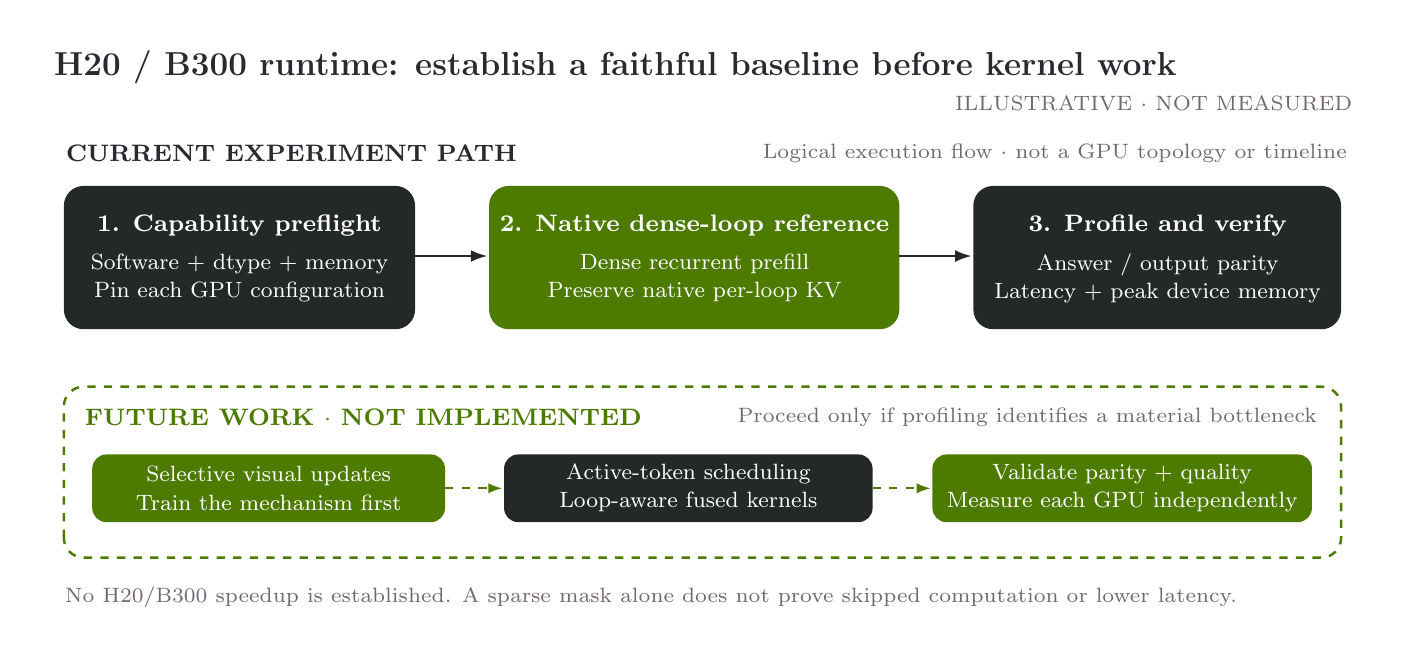
\begin{tikzpicture}[x=1cm,y=1cm]
\path[use as bounding box] (0,0) rectangle (17.145,7.66);
\fill[white] (0,0) rectangle (17.145,7.66);
\node[title] at (.33,7.16) {H20 / B300 runtime: establish a faithful baseline before kernel work};
\status{6.70}{muted}
\node[label,anchor=west] at (.48,6.07) {CURRENT EXPERIMENT PATH};
\node[sub,anchor=east] at (16.76,6.07) {Logical execution flow $\cdot$ not a GPU topology or timeline};
% Actual experimental reference path, alternating dark and filled-green boxes.
\fill[rounded corners=2.5mm,graphite] (.46,3.83) rectangle (4.92,5.65);
\node[label,text=white] at (2.69,5.15) {1. Capability preflight};
\node[text=white,align=center] at (2.69,4.48) {Software + dtype + memory\\Pin each GPU configuration};
\draw[flow,draw=graphite] (4.92,4.76)--(5.84,4.76);
\fill[rounded corners=2.5mm,green] (5.86,3.83) rectangle (11.07,5.65);
\node[label,text=white] at (8.47,5.15) {2. Native dense-loop reference};
\node[text=white,align=center] at (8.47,4.48) {Dense recurrent prefill\\Preserve native per-loop KV};
\draw[flow,draw=graphite] (11.07,4.76)--(11.99,4.76);
\fill[rounded corners=2.5mm,graphite] (12.01,3.83) rectangle (16.68,5.65);
\node[label,text=white] at (14.35,5.15) {3. Profile and verify};
\node[text=white,align=center] at (14.35,4.48) {Answer / output parity\\Latency + peak device memory};
% Future work is separated rather than blended into the shipped path.
\fill[rounded corners=2.5mm,fill=white,draw=green,dashed,line width=.9pt] (.46,.93) rectangle (16.68,3.10);
\node[label,text=green,anchor=west] at (.72,2.71) {FUTURE WORK $\cdot$ NOT IMPLEMENTED};
\node[sub,anchor=east] at (16.38,2.71) {Proceed only if profiling identifies a material bottleneck};
\fill[rounded corners=1.8mm,green] (.82,1.38) rectangle (5.30,2.24);
\node[text=white,align=center] at (3.06,1.81) {Selective visual updates\\Train the mechanism first};
\draw[control,draw=green] (5.30,1.81)--(6.03,1.81);
\fill[rounded corners=1.8mm,graphite] (6.05,1.38) rectangle (10.73,2.24);
\node[text=white,align=center] at (8.39,1.81) {Active-token scheduling\\Loop-aware fused kernels};
\draw[control,draw=green] (10.73,1.81)--(11.47,1.81);
\fill[rounded corners=1.8mm,green] (11.49,1.38) rectangle (16.31,2.24);
\node[text=white,align=center] at (13.90,1.81) {Validate parity + quality\\Measure each GPU independently};
\node[sub,anchor=west] at (.47,.43) {No H20/B300 speedup is established. A sparse mask alone does not prove skipped computation or lower latency.};
\end{tikzpicture}
\end{document}
